% !TEX root = ../Thesis.tex
% !TEX spellcheck = en-US

\chapter{Emulation and simulation}
\label{ch:emulsimvirt}

Providing a precise definition, or ``definition framework'' for distinguishing simulators from emulators and why \emph{emulation} (as opposed to \emph{simulation}) is the focus of this dissertation is paramount.
In the literature, Wikipedia, or common dictionaries, there are contradictory definitions, overlapping concepts, and, in general, a vague distinction between the two is presented [INSERT MANY CITATIONS]. % TODO find and insert citations
That is why, rather than universally establishing what an emulator and a simulator are, it is intended that when, throughout this text, software package $A$ is an emulator and $B$ is a simulator in this or that sense, the reader can know without ambiguity what is meant.

\section{Simulator}
\label{sec:simulator}

A network simulator is a computer program (or software package) that implements algorithms corresponding to mathematical formulae and models of computer networks, and which allows, through any interface ---such as a graphical one---, designing, testing, analyzing, and observing the expected behavior of protocols, nodes, and links according to several parameters. Therefore, it allows for the study of routing (in the sense of ``planing'' routes) and switching (in the sense of making packets follow a given route at step of a path) protocols.

Even though the usefulness of these tools cannot be questioned, and some like Cisco Packet Tracer~\footnote{\url{https://www.netacad.com/courses/packet-tracer/introduction-packet-tracer}} are very used in the training of professionals in the networks administration and engineering fields, it is crucial to point out as the distinctive characteristic of simulators, as defined here, the fact that those applications constitute a ``closed'' universe in the sense of only \emph{simulating} events that change the status of internal data structures, but do not implement a real stack of protocols, where every operation that should be performed is, in fact, performed. % TODO this is super "Portuguese in English". Improve
The consequence is that these systems do not inter-operate with nodes from the outside.

In other words: a network simulator is a black box for the outside, with a set of available inspection and state alteration operations---i.e. that provides the ability to see some aspects of the simulated network and perform some finite set of changes to the simulated environment.
However, as long as the \emph{implemented} cause-effect behaviors for that set of operations \emph{is coherent} to their real-world counterparts, any kind of ``shortcuts'' inside can be taken.

\section{Emulator}
\label{sec:emulator}

The definition for an emulator can, therefore, pretty much be inferred from the simulator as its ``complement''.
Software computer network emulators are solutions that allow, without resorting to the usage of physical equipment (even though sometimes allow for it, if desired) prototyping networks for analysis and study of underlying mechanisms, investigation, and development of new protocols and solutions, etc., thanks to an array of techniques that can span from virtualization and containerization, hardware architecture emulation, and leveraging operating system functionality in multi-process environments.

Unlike the aforementioned simulators, the fact of the traffic being real (at least from a logical standpoint) and that is possible to ``glue'' emulated interfaces with any kind of physical ones detected by the host operating system, offers the possibility of mixing emulated topologies with real topologies, cloud machines, etc.
Besides, since the computational nodes (hosts in the emulated topologies) are containers or VMs, running real software, the limit in terms of what it is possible to configure, parameterize, implement, or test, for any stack level (from the link to the application layer) is theoretically nonexistent.

\section{The comparison and the continuum from ``the reality'' to simulators}
\label{sec:emulationversussimulation}

\begin{figure}
  \centering
  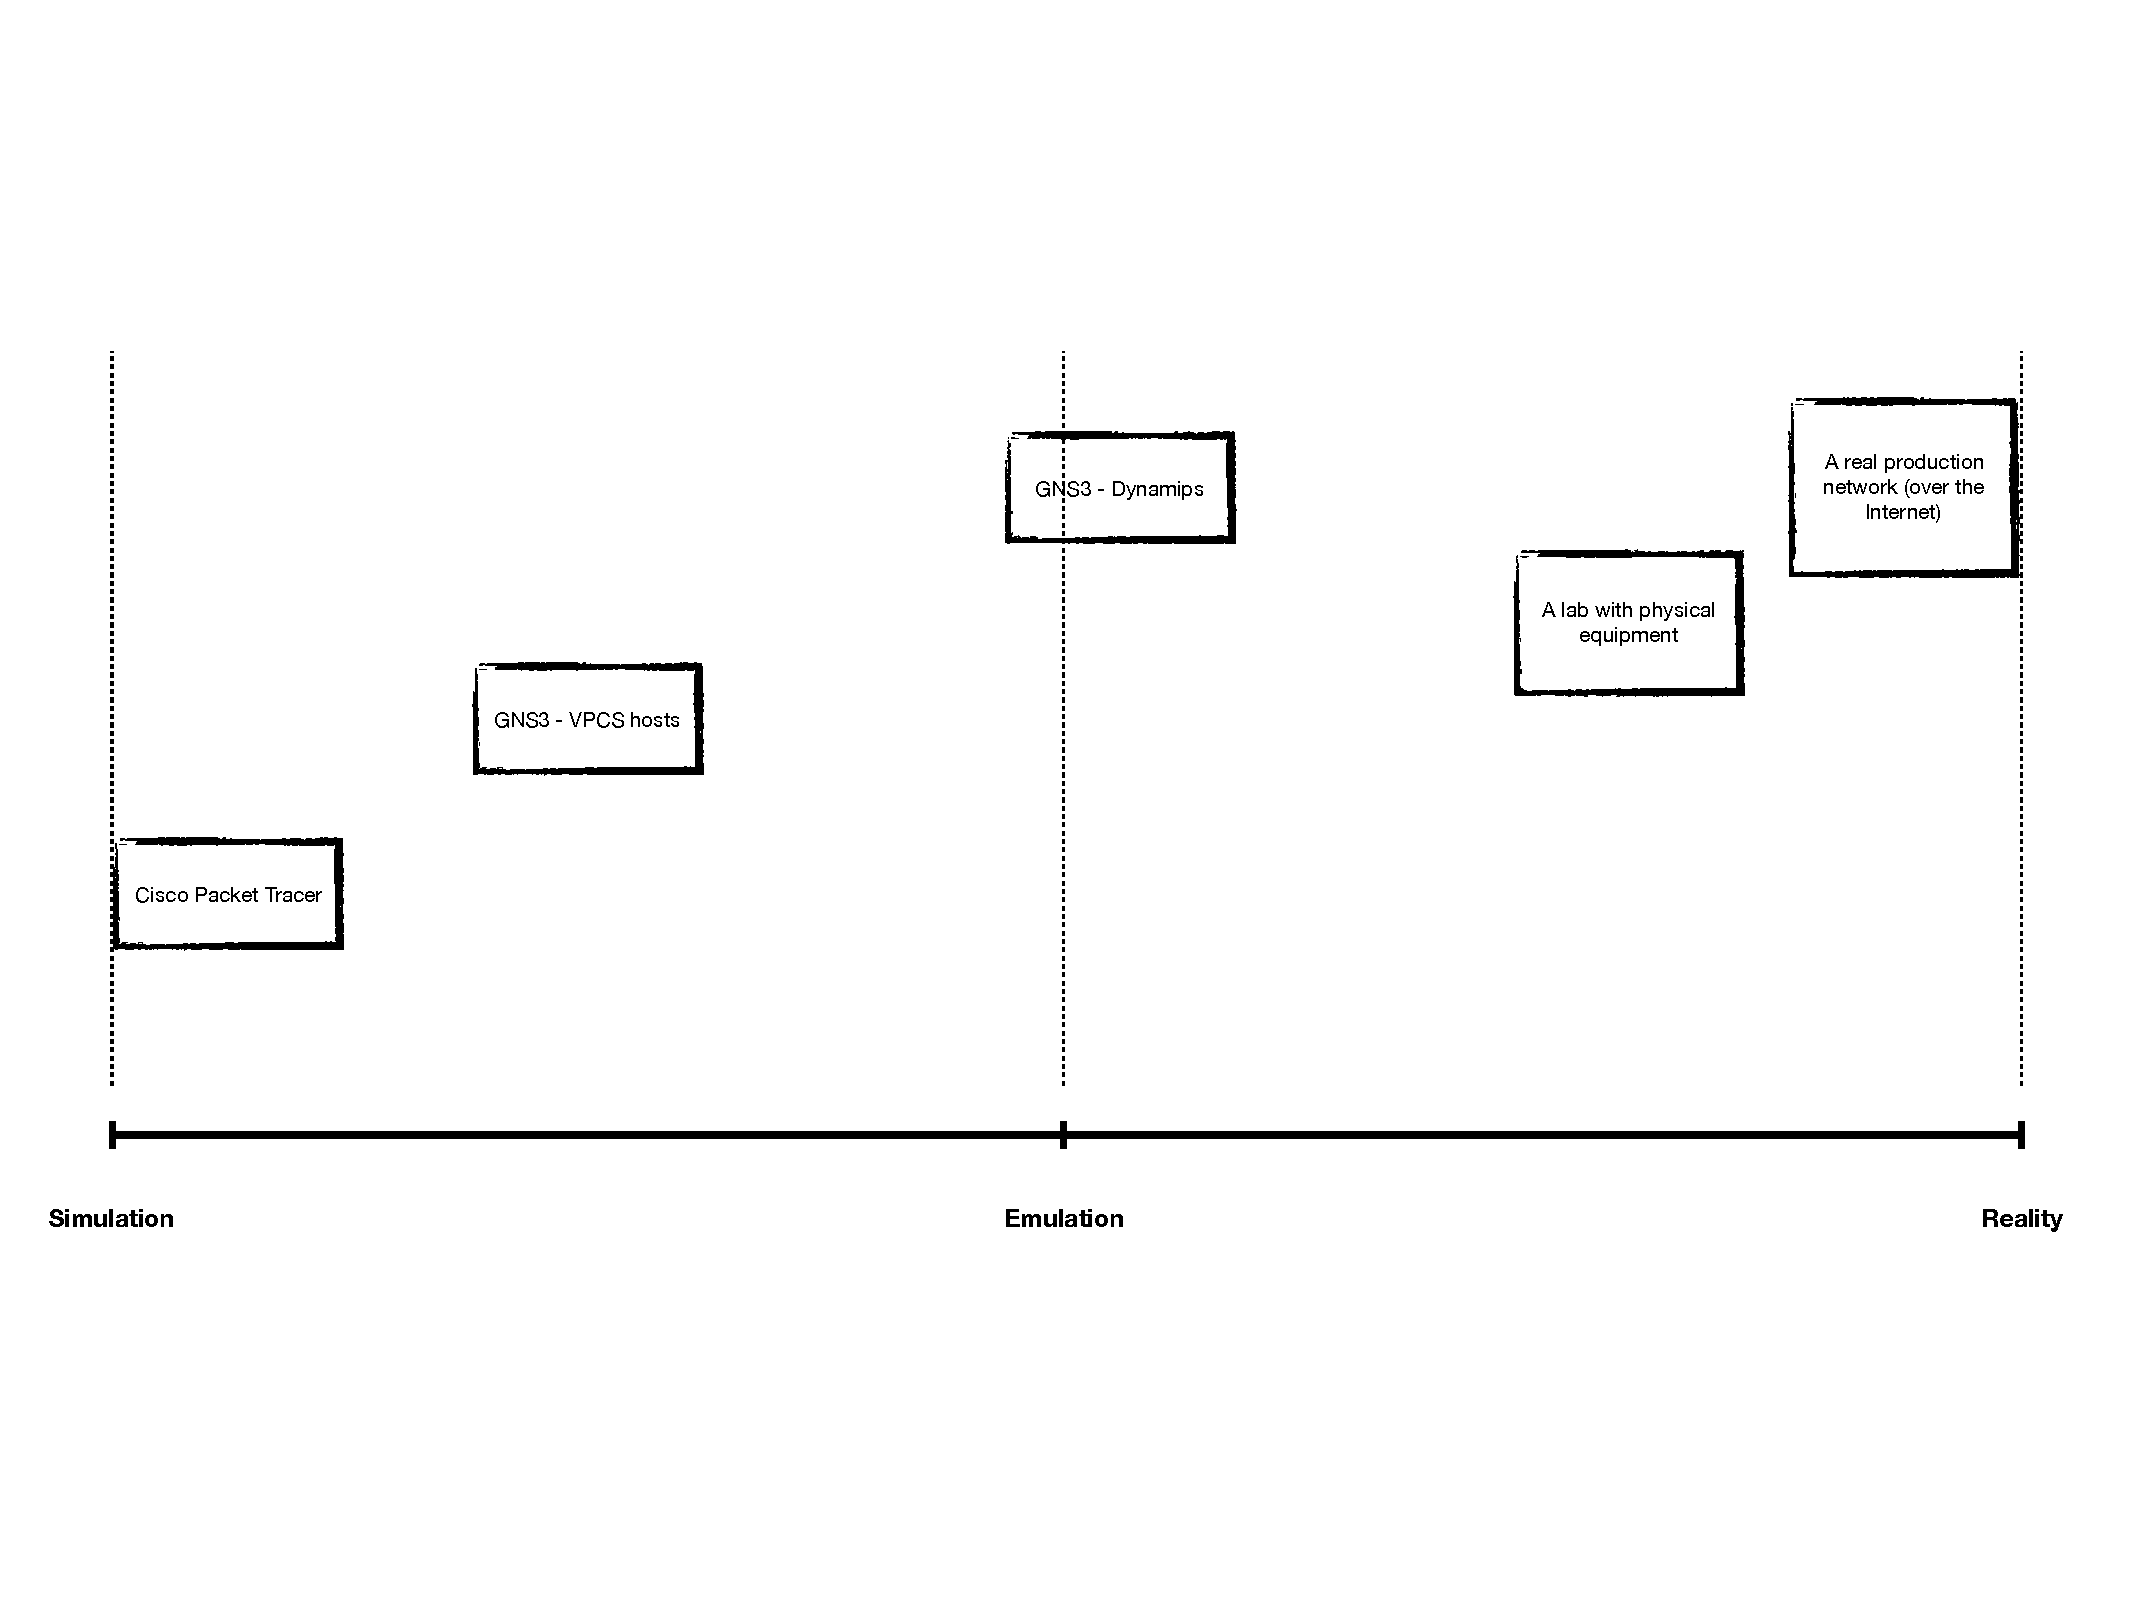
\includegraphics[width=0.8\textwidth]{emulationvsreality}
  \caption{Simulation vs emulation vs reality}
  \label{fig:emulationvsreality}
\end{figure}

What both have in common is that they are ways of providing students, researches, developers, administrators, or any professional that works with computer networks with an alternative to the real network that is being studied, for convenience and/or cost effectiveness. However, a lab with network nodes in an education institution is also different from the reality it is trying to model. That idea is exposed in the diagram in figure~\ref{fig:emulationvsreality}.

On one end there is reality---factors like amount of nodes, physical length of links (and therefore propagation times) can only be \textbf{simulated} in a lab, let alone on an solution that is fully software-based, like the emulators described in section~\ref{sec:emulator}. An anecdote like the 500-mile email~\footnote{The case of the 500-mile email~\cite{500mileemail} was an issue described by a systems administrator where e-mails could not be sent to servers further than 500 miles.
The description seemed impossible as e-mail servers (closer) were working, but a hidden configuration---a timeout---rendered a different behavior according to the physical distance between hosts, due to round-trip times.
} could not be reproduced, without simulating an---then---unknown ``flaw'', in an emulator consisting in virtual machines running the real software and performing the real operations---the cause of the problem was latency.

On the other end there is full simulation, where nothing is real.

In the middle, complex solutions like GNS3, which is presented in great detail in chapter~\ref{ch:gns3}, can offer a mixture, while being mainly emulators in the sense that it consists in an orchestrated set of processes running the real code, and also allowing to simulate aspects of reality like failures in links and delays.

The reason why emulators are specially interesting and are essentially the motivation (\ref{sec:motivation}) of this work, though, is that giving away the lab room with its switches and cables requires to not lose the flexibility it offers to perform all kind of pedagogical exercises, and ``pure'' simulators do not offer by inherent limitation.
